\chapter{AI datacenter networking}
\label{ch:networking}

Optics only make sense once you see the fabric they sit in. Training and
inference clusters are not one network; they are several overlapping networks
with different bandwidth, latency, and reach needs. This chapter places the
devices and validation methods from earlier chapters into that system context:
how AI clusters are wired, why the interconnect sits on the inference critical
path, and where optics dominates cost and power.

\section{Scale-up versus scale-out}
\label{sec:scale-up-out}

The industry borrowed two words from computer architecture and overloaded them
for AI fabrics. Keeping them straight matters, because they buy different optics.

\begin{description}
\item[Scale-up] tight coupling inside a node or rack: GPU-to-GPU over a
      memory-semantic fabric (for example NVLink). Very high bandwidth, very low
      latency. Increasingly optical as bandwidth outgrows copper reach.
\item[Scale-out] coupling across racks and pods over a switched network
      (Ethernet or InfiniBand). This is where pluggable and co-packaged optics
      have long lived.
\end{description}

\begin{figure}[ht]
\centering
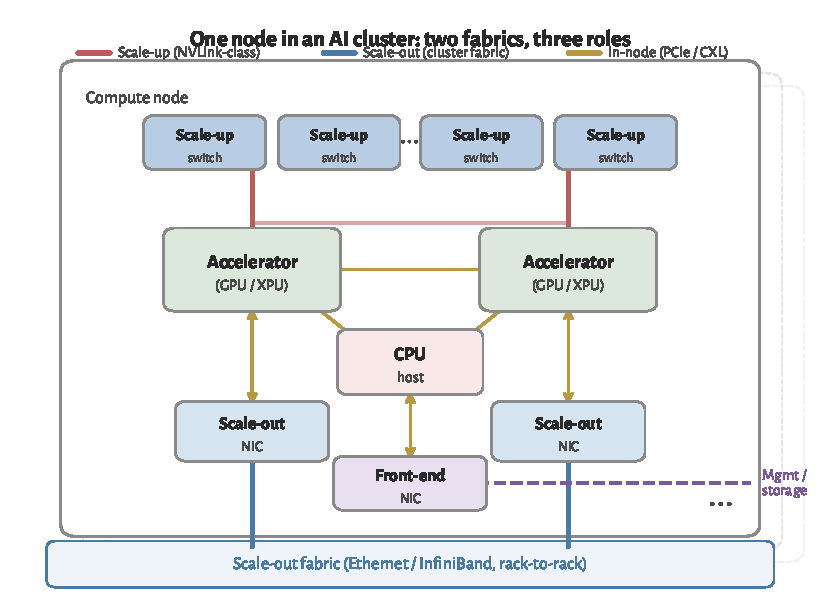
\includegraphics[width=\linewidth]{figures/fig_scale_up_node.pdf}
\caption{Schematic AI compute node (one tray in a larger cluster). \emph{Accelerators}
         are the heavy compute engines (typically GPUs; the book also uses XPU for
         GPUs and custom ASICs). \textbf{Scale-up} links (red) tie accelerators through
         a high-bandwidth, low-latency switch fabric inside the node or rack
         (NVLink-class). \textbf{Scale-out} links (blue) leave via a dedicated NIC
         per accelerator into the datacenter Ethernet or InfiniBand fabric.
         The CPU and front-end NIC handle host, storage, and management traffic.\label{fig:scale-node}}
\end{figure}

\subsection{Three networks, two that set the optics budget}

The OIF CEI-448G framework names \emph{three} distinct networks in a large AI
cluster~\firstcite{cei448}. \Cref{fig:scale-node} shows two; the third is easy to
overlook:

\begin{description}
\item[Scale-up] accelerator-to-accelerator inside a pod or rack. Highest bandwidth
      per link, lowest latency, often lossless. Dominates compute time if under-
      provisioned.
\item[Scale-out] accelerator-to-accelerator (or node-to-node) across the cluster
      over a switched fabric (InfiniBand, \term{UEC}\firstterm{UEC}/Ethernet with
      RoCE or Ultra Ethernet Transport). Lower per-link bandwidth than scale-up,
      but must reach $10^5$+ endpoints.
\item[Front-end] CPU-attached traffic: management, control plane, checkpointing,
      storage, and training-data ingest. Analogous to a conventional cloud
      datacenter network; not the IM/DD bottleneck this book focuses on, but it
      shares the same rack power and cabling budget.
\end{description}

Scale-up carries the majority of \emph{interconnect} bandwidth inside a training
job; scale-out multiplies link count across the building. That is why both push
448G-class lane rates and why optics shows up first on scale-out, then on
scale-up as copper reach shrinks~\firstcite{cei448}.

\subsection{Scale-up versus scale-out at a glance}

\Cref{tab:oif-scale} condenses OIF Table~1 (CEI-448G framework, \S2.2): order-of-
magnitude targets for node count, physical extent, and media type~\firstcite{cei448}.
Numbers are industry snapshots, not hard limits, but they explain why ``optics
inside the rack'' and ``optics between racks'' arrive on different timelines.

\begin{table*}[ht]
\refstepcounter{table}\label{tab:oif-scale}%
\centering
\setlength{\tabcolsep}{4pt}%
\footnotesize
\begin{tabular}{@{}p{0.22\linewidth}p{0.17\linewidth}p{0.17\linewidth}p{0.17\linewidth}p{0.17\linewidth}@{}}
\toprule
 & \multicolumn{2}{c}{Scale-up} & \multicolumn{2}{c}{Scale-out} \\
\cmidrule(lr){2-3}\cmidrule(lr){4-5}
Metric & Today & Next gen & Today & Next gen \\
\midrule
Accelerator nodes in domain & $\sim$100 & $\sim$1\,k & 100\,k+ & $\gg$100\,k \\
Physical extent & Rack & Rack to row & Datacenter & Datacenter \\
Network properties & \multicolumn{2}{p{0.34\linewidth}}{Lossless, low latency} &
  \multicolumn{2}{p{0.34\linewidth}}{Large scale; multi-tier switching} \\
Media within rack &
  \multicolumn{2}{p{0.34\linewidth}}{Electrical: passive PCB / twinax backplane} &
  \multicolumn{2}{p{0.34\linewidth}}{Electrical: twinax backplane} \\
Media between racks &
  AEC (adjacent racks) & Optical (within row) &
  \multicolumn{2}{p{0.34\linewidth}}{Optical (pluggable or CPO on switch/NIC)} \\
\bottomrule
\end{tabular}
\par\medskip
{\raggedright\footnotesize\textbf{Table~\thetable.} Scale-up vs.\ scale-out
snapshots (adapted from OIF CEI-448G framework Table~1, 2025). Scale-up stays
on copper as long as rack densification keeps channels short; scale-out is already
optical at datacenter scale.\par}
\end{table*}

\subsection{Standards bodies: who owns what}

448G/lane signaling is not owned by one standards body, and that is by design.
Electrical reach, Ethernet naming, connectors, and rack packaging evolved in
different rooms; AI fabrics forced them to meet at the same lane rate. OIF's
CEI-448G framework (\S2.3) lists the groups that must align~\firstcite{cei448}.
\Cref{tab:sdo-map} maps each body to the layer an optical engineer actually
touches. The short version: OIF sets the electrical baud and reach classes; IEEE
names the Ethernet optical PMD; UALink and UEC own scale-up and scale-out
protocol stacks; SNIA and OCP decide connectors and where the optics physically
live. The \term{LPO MSA} is not a standards body, but it publishes the only open
end-to-end spec that stitches CEI Linear electrical limits to IEEE optical PMD
limits for DSP-less modules (\Cref{sec:lpo-msa}). Prose below expands each OIF
summary.

\begin{table*}[ht]
\refstepcounter{table}\label{tab:sdo-map}%
\centering
\setlength{\tabcolsep}{5pt}%
\footnotesize
\begin{tabular}{@{}p{0.12\linewidth}p{0.14\linewidth}p{0.70\linewidth}@{}}
\toprule
Body & Fabric & What matters for short-reach optics \\
\midrule
OIF CEI & All reaches & Electrical PHY: XSR/VSR/MR/LR, 448G PAM4/6/8, LPO/LRO; CMIS for module management \\
UALink & Scale-up & Open load/store pod fabric; 200G/lane today, $\sim$400G/lane next; drives XSR-class PHY needs \\
UEC & Scale-out & Ultra Ethernet Transport, congestion control; PHY group surveying 400G/lane enhancements \\
SNIA SFF & Host / backplane & Cables, connectors, PCIe/EDSFF form factors; SFF 448G COM for backplane (complements CEI front-panel work) \\
OCP & Rack / system & Open rack designs, CPO/XPO placement, optical circuit switching (OCS) for AI clusters \\
IEEE 802.3 & Scale-out (+ optics PMD) & Ethernet MAC rates (802.3dj, 400G/lane SG), KP4 FEC, IM/DD PMD clauses (DR/FR, TDECQ) \\
\bottomrule
\end{tabular}
\par\medskip
{\raggedright\footnotesize\textbf{Table~\thetable.} SDO roles at 448G/lane (after OIF CEI-448G \S2.3).\par}
\end{table*}

\paragraph{OIF.} Common Electrical I/O (\term{CEI}) Implementation Agreements are
the modular electrical PHY recipes: die-to-die (\term{XSR}), chip-to-module
(\term{VSR}), chip-to-chip (\term{MR}), and backplane (\term{LR}). CEI-448G is
the current AI-driven push beyond 224G/lane~\firstcite{cei448}. Related OIF tracks
include energy-efficient interfaces (EEI), CMIS management extensions at 448G,
and coherent DCI (out of scope for this book). For optics, CEI tells you the
\emph{baud and reach} the module or CPO engine must meet; IEEE 802.3 tells you
how Ethernet names the optical PMD.

\paragraph{UALink Consortium.} \term{UALink}\firstterm{UALink} specifies an open \emph{scale-up}
stack (transaction, data link, and physical layers) optimized for direct
accelerator memory access, not IP/Ethernet~\firstcite{ualink200,cei448}. UALink
1.0 targets 200G/lane and pods up to roughly 1\,k accelerators; the physical-layer
working group is gathering requirements for $\sim$400G/lane. Optical engineers
care because higher lane rate reduces port count on the accelerator package, and
because scale-up eventually hits the same copper reach wall as CEI XSR
(\Cref{sec:trace-loss}).

\paragraph{Ultra Ethernet Consortium.} \term{UEC} builds a complete Ethernet-based
stack for AI/HPC \emph{scale-out}: transport (UET), link layer, and PHY
enhancements~\firstcite{uec10,cei448}. UEC 1.0 (June 2025) targets cluster-scale
congestion control and RDMA-class performance over standard Ethernet hardware,
including NICs, switches, optics, and cables. The PHY working group is surveying
400G/lane improvements. This is the protocol layer above the transceiver; IM/DD
module specs still come from IEEE and MSAs.

\paragraph{SNIA (SFF Technology Affiliate).} SNIA's SFF working group defines
connectors, cables, and form factors for storage and compute backplanes, not
front-panel Ethernet~\firstcite{snia448,cei448}. The SFF 448G project
(SFF-TA-1043) parallels CEI-448G but focuses on backplane COM, package insertion
loss, and PAM choice on copper channels inside the box. Pair OIF VSR (module
connector) with SFF (host PCB and PCIe cable) when debugging a link budget.

\paragraph{Open Compute Project.} OCP publishes open rack, server, and networking
designs for hyperscale~\firstcite{ocpai,cei448}. Relevant work includes Open
Systems for AI, short-reach optical interconnect guidelines, and the Optical
Circuit Switching (OCS) subproject (2025) for reconfigurable cluster fabrics.
OCP rarely specifies baud rate; it specifies \emph{where} the optical engine
lives (faceplate pluggable vs.\ CPO vs.\ XPO) and how it is cooled and serviced.

\paragraph{IEEE 802.3.} Ethernet standards define MAC rates, FEC (KP4 in
Clause~91), and interoperable optical PMDs~\firstcite{ieee8023dj,e4ai448,cei448}.
802.3dj (200G/lane) and the 400G/lane study group name the product generations
that consume 224G and 448G-class optics. One naming trap: IEEE quotes
\textbf{400~Gb/s per lane} (MAC/info rate); CEI quotes \textbf{$\sim$448~Gb/s}
(line rate with coding overhead). Same physics, different accounting
(\Cref{ch:imdd,tab:rate-stack}).

The frontier is optics entering the scale-up domain (optical NVLink-class links,
co-packaged switches), because copper reach at 200G/lane is only about a meter.

\section{Topologies and why optics count explodes}
\label{sec:topologies}

Cluster topology is where optical count stops being ``a few modules per server''
and becomes a fleet problem. Large AI fabrics mostly use fat-tree / Clos,
rail-optimized, or dragonfly layouts. In a classic $k$-ary fat-tree, link count
scales as $O(k^3)$ while endpoints scale as $O(k^2)$: optics multiply faster than
compute. Rail-optimized designs (one NIC rail per accelerator row, all-to-all
within a rail) rose with collective-heavy training and inference because they cut
oversubscription on all-reduce paths, at the price of more parallel optical
planes. Dragonfly and other hierarchical topologies trade some global bisection
bandwidth for fewer long links.

The optical engineer cares because every topology choice sets link count, which
sets laser count, module count, and FIT budget (\Cref{ch:reliability}); rail
layouts drive fan-out from leaf to spine and push denser 800G/1.6T ports toward
CPO/XPO (\Cref{sec:cpo-status,sec:xpo}); and scale-up inside the rack stays
electrical longer while scale-out between racks is already optical
(\Cref{tab:oif-scale}). That explosion in link count is the economic reason a
hyperscaler builds an in-house optical engineering team.

\section{Pluggable form factors and module styles}
\label{sec:pluggables}

Faceplate modules differ in aggregate rate, lane count, electrical reach, and
where the DSP lives. The form factor sets the passive channel the SerDes must
survive, and the last decade of AI networking has mostly been a fight over that
choice: keep a retimer in the module for interop, delete it for watts (LPO/LRO),
or move the optics onto the package (CPO) and service the laser from the
faceplate (ELSFP).

\begin{description}
\item[QSFP-DD / OSFP] the incumbent datacom pluggables. QSFP-DD carries 800G/1.6T
      class products (eight lanes at 100G or 200G per lane). OSFP targets higher
      power and density (1.6T today, 3.2T roadmaps) with a larger cage and better
      thermal path. Both impose a VSR-class electrical channel from host PCB through
      the connector (\Cref{sec:trace-loss,sec:conditioning}).
\item[Retimed module] DSP/CDR inside the module (\Cref{sec:equalization}). Default
      for interoperability; $\sim$15--20~W class at 800G/1.6T.
\item[LPO / LRO] linear or lightly retimed: delete or slim module DSP
      (\Cref{sec:conditioning,sec:drivers,fig:oif-448g-package,fig:eq-chains}). Power drops to $\sim$7--9~W but host
      EQ and transmitter and dispersion eye closure quaternary (TDECQ) margin
      tighten.
\item[ELSFP / external laser] field-replaceable CW source for CPO
      (\Cref{sec:cpo-status,ch:lasers}): decouples laser FIT from switch FIT.
\item[XPO] liquid-cooled mega-pluggable (\Cref{sec:xpo}): 12.8~Tb/s per module,
      front-panel serviceability with CPO-class density.
\end{description}

\term{CMIS} (\Cref{sec:cmis}) is the management layer for module identity, monitors,
and (at 224G/448G) link-training and host-side signal-integrity tuning extensions.
Optical engineers touch it when debugging lock, FEC, and equalizer settings across
vendors.

\paragraph{Half-retimed and asymmetric modules.}
\label{sec:module-styles}

Not every pluggable is fully retimed or fully linear. Common 2025--26 variants
sit between those poles:

\begin{description}
\item[LPO] linear drive and linear receive: no module DSP/CDR
      (\Cref{sec:equalization,sec:drivers}).
\item[LRO / RTLR] retimed transmit, linear receive (OIF RTLR): DSP on electrical
      $\to$ optical only; eases host TX while keeping a simpler RX path~\cite{lpo}.
\item[TRO / half-retimed] symmetric opposite or partial retiming variants appear in
      vendor roadmaps; always check which direction carries the DSP.
\item[Fully retimed] DSP both directions; default for interoperability at 800G/1.6T.
\end{description}

Power scales with DSP content: retimed $\sim$15--20~W, LRO $\sim$9~W, LPO
$\sim$7--9~W at 800G class (\Cref{sec:power}). The architecture choice is a trade
between host margin (COM, TDECQ) and module watts.

\subsection{The LPO MSA: stitching IEEE optics to CEI Linear}
\label{sec:lpo-msa}

OIF CEI tells you the electrical recipe at the module cage. IEEE 802.3 tells you
how Ethernet names the optical PMD and its TDECQ/OMA limits. Neither document,
by itself, is a complete product spec for a linear pluggable that deletes the
module DSP. The \term{LPO MSA}\firstterm{LPO MSA} (Linear Pluggable Optics
Multi-Source Agreement) fills that gap: one open specification for both sides of
the module, with normative test points and host responsibilities spelled
out~\firstcite{lpomsa,lpo}.

The first published revision, \emph{100G-DR-LPO} (v1.0, March 2025), targets
100~Gb/s per lane at 53.125~GBd PAM4 on single-mode fiber from 0.5~m to 500~m.
It is explicitly a data-center profile: low power, low latency, high port density,
RS(544,514) FEC on the host, and form-factor agnostic (QSFP, QSFP-DD, OSFP are
examples, not the spec). The naming pattern generalizes to \texttt{n00G-DRn-LPO}
for $n\in\{1,2,4,8\}$ lanes. Optical reach and modulation track IEEE DR-class
PMDs; the electrical interface tracks OIF CEI-112G-LINEAR-PAM4. That split is the
template 224G linear modules follow: CEI-224G-Linear on the AUI, 802.3dj optical
PMD limits on the fiber (\Cref{sec:224g-deploy,sec:pmd-reach}).

\paragraph{Who owns which block.}
In an LPO link the host is not a passive cable driver. It runs KP4 FEC
(\Cref{sec:kp4}), full SerDes equalization (CTLE, FFE, DFE, CDR;
\Cref{sec:equalization,sec:serdes-dsp}), and optional nonlinear compensation
(NLC) and startup protocol functions. The module is analog: linear driver,
modulator or laser, photodiode, TIA, and at most a fixed CTLE. No retiming, no
FEC, no heavy DSP. CMIS (\Cref{sec:cmis}) is the management contract. SFF
hardware specs (QSFP-DD, OSFP cages) set the mechanical envelope. The MSA's job
is to define what must pass at each interface between those blocks so modules
from different vendors close on the same host.

\paragraph{The test-point ladder.}
LPO MSA normative compliance is organized around six electrical/optical test
points (\Cref{tab:lpo-tp}). Think of them as the validation script: host TX at
TP1a, module optical TX at TP2, stressed optical RX at TP3, module electrical RX
at TP4, and stressed host RX at TP4a. Section~10 of the MSA adds a host-to-host
end-to-end BER test with FEC-encoded traffic, which is how you prove interop after
the point tests pass.

\begin{table}[ht]
\centering
\caption{LPO MSA test points (100G-DR-LPO).\label{tab:lpo-tp}}
\setlength{\tabcolsep}{4pt}%
\footnotesize
\begin{tabular}{@{}p{0.08\linewidth}p{0.30\linewidth}p{0.54\linewidth}@{}}
\toprule
Point & Location & Principal measurements \\
\midrule
TP1a & Host SerDes output & EECQ (electrical eye closure), host TX quality \\
TP1 & Module electrical input & Module input stressor calibration \\
TP2 & Optical TX (2--5~m patch cord) & TDECQ, TECQ, OMA$_{\mathrm{outer}}$, RIN$_{x\mathrm{OMA}}$, ER \\
TP3 & Optical RX input & Stressed receiver calibration (SECQ), sensitivity masks \\
TP4 & Module electrical output & Module RX linear output (EECQ) \\
TP4a & Stressed host input & Host RX under worst-case module output \\
\bottomrule
\end{tabular}
\end{table}

\paragraph{Optical limits that matter.}
The MSA optical tables (\Cref{sec:tdecq,ch:validation}) inherit IEEE 802.3
measurement methods with LPO-specific reference equalizers. The numbers you will
quote in a datasheet review:

\begin{itemize}
\item TDECQ and TECQ capped at 3.4~dB per lane, measured with a 9-tap T-spaced
      reference FFE and SER target $4.0\times10^{-4}$.
\item OMA$_{\mathrm{outer}}$ coupled to transmitter quality: launch power in OMA
      rises with max(TECQ, TDECQ) along a piecewise mask (for example
      $-3.2 + \mathrm{max}(\mathrm{TECQ},\mathrm{TDECQ})$~dBm in the mid-TECQ
      region).
\item RIN$_{x\mathrm{OMA}} \le -138$~dB/Hz at 17.2~dB ORL (the ``$x$'' subscript
      tracks return loss, same convention as IEEE DR PMDs).
\item Illustrative link budget 6.7~dB total at 500~m (3~dB channel loss plus 0.3~dB
      MPI penalty plus 3.4~dB TDECQ allocation).
\item Stressed receiver sensitivity $-3.1$~dBm OMA$_{\mathrm{outer}}$ at TP3 with
      SECQ = 3.4~dB and aggressor lanes at 4.2~dBm OMA.
\end{itemize}

TECQ is TDECQ without the dispersion test fiber. The MSA uses both because outer
OMA limits are written against max(TECQ, TDECQ), and a module can be fiber-limited
even when the electrical eye looks clean.

\paragraph{Electrical limits and host COM.}
On the electrical side the MSA points to CEI-112G-LINEAR-PAM4 for the host-to-module
interface and defines EECQ (electrical eye closure quaternary) at TP1a and TP4a.
That is the electrical analogue of TDECQ: a host that passes optical TDECQ at TP2
but fails EECQ at TP1a still will not interoperate. Host PCB insertion loss,
connector, and module input return loss sit in the channel reference model
(Section~7). For 224G deployment, swap CEI-112G-LINEAR for CEI-224G-Linear and run
the same two-ledger program (\Cref{sec:224g-deploy,sec:com}).

\paragraph{What to read first.}
For a bring-up engineer the reading order is: Section~5 (system overview and host
FEC requirements), Section~7 (electrical TPs and channel model), Section~8
(optical TX/RX tables), Section~9 (parameter definitions, especially 9.5 TDECQ/TECQ
and 9.10 stressed RX), then Section~10 (host-to-host FEC BER). Cross-check every
optical definition against the cited IEEE 802.3 clause; the MSA adds reference
equalizer taps and SER targets, not new physics.

\keyidea{OIF owns the electrical baud at the cage. IEEE owns the optical PMD
metrics on the fiber. The LPO MSA is the product contract that binds them for
DSP-less modules: normative test points, host FEC/EQ duties, and TDECQ/OMA masks
you can test without a module retimer safety net.}

\section{Emerging link styles}

The form-factor list above is the present. The industry argument for 2025--26 is
where the DSP and the laser should live next. Retimed pluggables remain the
interop default: a module DSP cleans the electrical channel, at the cost of
watts. LPO and LRO delete or slim that DSP so the host SerDes carries more of the
EQ burden, which is attractive for AI power budgets and painful for margin and
interop. CPO moves the optical engine onto the switch or XPU substrate to cut
electrical reach, and usually keeps the laser external and field-replaceable
(ELSFP/CW-WDM). XPO appeared in 2026 as a middle path: a much larger,
liquid-cooled pluggable that keeps front-panel serviceability while pushing
density toward CPO territory (\Cref{sec:xpo}). The rest of this chapter treats
electrical reach, eye budgets, and vendor CPO programs as consequences of that
argument.
\section{The electrical link: reach, conditioning, and the eye budget}
\label{sec:trace-loss}

Every form factor above is really an answer to one physical question: \emph{how far
can the electrical signal travel before it is cheaper (in power and dB) to convert
to light?} As the per-lane rate climbs, that distance collapses, and it is what
pushes the optics from the faceplate toward the die.

\newthought{Trace loss scales with frequency.} A PCB stripline's insertion loss
grows roughly with $\sqrt{f}$ (skin effect) plus a dielectric term linear in $f$,
so it is quoted per inch \emph{at the Nyquist frequency}. Going from 112G to 224G
PAM4 moves Nyquist from 28~GHz to 56~GHz, and the loss per inch roughly doubles.
Recent 224G board studies measure $\approx2.8$~dB/inch for regular stripline and
$\approx1.9$~dB/inch with skip-layer routing at 56~GHz, against a next-generation
\emph{target} of 1~dB/inch that demands ultra-low-loss dielectric, HVLP copper, and
short via stubs~\cite{traceloss}. \Cref{fig:traceloss} shows the consequence: at a
fixed PCB-trace budget, doubling the baud rate roughly halves the copper reach.

\begin{figure}[ht]
\centering
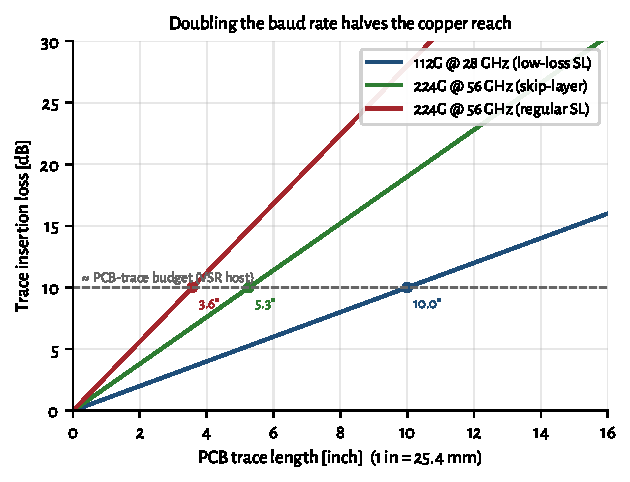
\includegraphics[width=\linewidth]{figures/fig_trace_loss.pdf}
\caption{PCB trace insertion loss versus length at each rate's Nyquist. The reach to
a fixed budget shrinks from $\sim\!10$ inches (112G) to a few inches (224G), which
is why the optical conversion must move closer to the ASIC.\label{fig:traceloss}}
\end{figure}

\newthought{The CEI channel classes name the reaches.} OIF's Common Electrical I/O
project defines the electrical link budgets the whole industry designs to.
\Cref{tab:cei224-reach} is the CEI-224G lookup card (XSR / VSR / MR / LR, plus
Linear for DSP-less modules); the reach map is \Cref{fig:cei-reach-map}. At
56~GHz Nyquist the same names mean much shorter copper than at 112G~\cite{cei224}:
\begin{description}
\item[XSR] \term{XSR}\firstterm{XSR}: die-to-die / die-to-engine: the shortest, lowest-power tier, the one CPO
      and chiplet optics live in ($\lesssim$50~mm package).
\item[VSR] \term{VSR}\firstterm{VSR}: chip-to-module: $\approx$200~mm of host plus 20~mm of module and one
      connector: the classic pluggable channel.
\item[MR] \term{MR}\firstterm{MR}: chip-to-chip across a board: $\approx$500~mm, one connector,
      $\sim$32--34~dB die-to-die.
\item[LR] \term{LR}\firstterm{LR}: backplane or copper cable: $\approx$1000~mm of host and daughter cards,
      two connectors, up to $\sim$40~dB die-to-die (including a 1~m cable).
\item[Linear] \term{CEI-224G-Linear}: same faceplate-class ports without a module
      DSP/CDR; the electrical foundation for LPO (\Cref{sec:224g-deploy,sec:pluggables}).
\end{description}

\paragraph{Active copper: ACC, AEC, and DAC.}
\label{sec:active-cables}

Passive direct-attach copper (DAC) survives only where the reach is short: at 224G a
passive DAC is good for roughly $0.5$--$1$~m (strong 224G PHYs have demonstrated
2~m). \term{ACC}\firstterm{ACC} adds redrivers (CTLE + VGA) in the cable; \term{AEC}\firstterm{AEC}
adds retimers (EQ + CDR) and stretches twinax to $\sim$2.5~m at higher power
(\Cref{sec:conditioning,sec:equalization})~\cite{dac224}. Beyond that, and
increasingly \emph{within} the rack for scale-up, the answer is optics
(\Cref{tab:oif-scale}).

\newthought{So the optics march inward.} Shortening the electrical path is exactly
what trades power and reach for serviceability, the through-line of this chapter.
\Cref{tab:placement} lays out the ladder from faceplate to interposer.

\begin{table*}[ht]
\refstepcounter{table}\label{tab:placement}%
\centering
\setlength{\tabcolsep}{5pt}%
\begin{tabular}{@{}p{0.20\linewidth}p{0.22\linewidth}p{0.15\linewidth}p{0.30\linewidth}@{}}
\toprule
Placement & Host electrical reach & Energy/bit & Serviceability \\
\midrule
Pluggable (faceplate) & full VSR host run ($\sim$200~mm) + connector & highest ($>$30~pJ/bit w/ DSP; less for LPO) & hot-swap at faceplate (best) \\
On-board optics (OBO / COBO) & shorter mid-board trace & lower & board-level (solder/socket); largely bypassed for CPO \\
Near-packaged (NPO) & engine beside the ASIC on substrate & lower still & module on substrate; limited \\
Co-packaged (CPO) & mm-scale die-to-engine (XSR) & $<$5~pJ/bit & soldered; ELSFP lasers field-replaceable \\
Optical I/O on interposer & on-die / interposer & $<$2~pJ/bit & not field-serviceable (emerging) \\
\bottomrule
\end{tabular}
\par\medskip
{\raggedright\footnotesize\textbf{Table~\thetable.} The optics-placement ladder.
Moving the electro-optic conversion inward cuts trace loss and energy per bit but
erodes field serviceability, the central tension behind pluggables, OBO/NPO, CPO
(\Cref{sec:cpo-status}), and the XPO middle ground (\Cref{sec:xpo}). A mid-board
fiber connector can shift breakage risk from the costly engine to a cheap
jumper.\par}
\end{table*}

\newthought{On-board optics: the step the industry mostly skipped.} OBO (standardized
by the \term{Consortium for On-Board Optics}, COBO) moves the optical engine off the
faceplate and onto the main PCB, cutting the copper run without abandoning silicon
photonics~\cite{cobo}. It works, but it gives up hot-plug serviceability while only
partly closing the power gap, so with CPO maturing, most hyperscalers are leapfrog\-ping
OBO/NPO straight to co-packaging, keeping serviceability via field-replaceable lasers
(\Cref{sec:cpo-status}) and the XPO pluggable hedge (\Cref{sec:xpo}).

\subsection{Reshaping, retiming, and where the DSP lives}
\label{sec:conditioning}

To survive that lossy channel the signal is conditioned at several points
(\Cref{sec:equalization}), and it helps to keep two device classes distinct.\sidenote{Rule of thumb: a redriver
reshapes, a retimer rebuilds timing. Neither fixes reflections or a bad return
path.}

\begin{description}
\item[Redriver] an analog \emph{reshaper/amplifier}: a \term{CTLE}\firstterm{CTLE} plus a VGA. It sharpens and boosts the eye but has
      \emph{no} clock recovery, so it cannot reset accumulated jitter; it adds
      almost no latency. This is the active element in active copper cables (ACC)
      and on host boards used to stretch a marginal trace.
\item[Retimer] adaptive EQ \emph{plus} a \term{CDR}\firstterm{CDR} that re-samples and regenerates the
      data. It breaks the channel into independent jitter/loss segments, at the
      cost of power and per-hop latency. Retimers sit in active electrical cables
      (AEC) and in fully retimed modules (Broadcom's Agera is a host retimer).
\end{description}

Inside the optical module the traditional ``cleanup'' is a full DSP (retimer $+$
FEC engine). The retimed-to-linear spectrum trades exactly cleanup for power and
latency:
\begin{description}
\item[Fully retimed] DSPs in both directions: least sensitive to \term{ISI}\firstterm{ISI}/dispersion,
      but highest power ($\sim$14--18~W/module at 800G) and most latency
      ($\sim$8--10~ns/hop).
\item[LPO (linear)] \term{LPO}\firstterm{LPO}: \emph{no} DSP or CDR in either direction: only a CTLE in the
      TIA and a linear driver, so the host SerDes must do all the \term{FFE}\firstterm{FFE}/CTLE
      equalization \emph{and} carry the FEC. Lowest power ($\sim$7--9~W), lowest
      latency ($<$3~ns), but most ISI/dispersion-sensitive and shortest reach
      ($<$2~km)~\cite{lpo}.
\item[LRO / TRO (retimed TX, linear RX)] DSP only on the electrical$\to$optical
      path, roughly half the power, sensitivity, and latency, with easier interop.
\end{description}

So yes: reshapers/amplifiers (redrivers) and retimers are routinely placed on the
host path, and the module's own DSP is the last line of cleanup. The entire LPO bet
(\Cref{sec:power,sec:224g-deploy}) is to \emph{delete} those active stages and let the host SerDes'
CTLE/FFE carry the channel, trading electrical margin for power and latency.

\subsection{The electrical eye: acceptable voltage and noise}
\label{sec:eye-budget}

What must the signal actually look like where it hands off to the module? The
CEI-224G reference and draft numbers set the envelope~\cite{cei224}. Differential
swing sits roughly in the 0.36--1.05~V\textsubscript{ppd} band (reference TX near
1~V peak-to-peak differential; lossier channels use the larger swing). Transmitter
\term{SNDR}\firstterm{SNDR} ($\mathrm{SNR_{TX}}$) is about 33~dB: the transmitter's own
noise-plus-distortion ceiling. PAM4 level uniformity needs
$\mathrm{RLM}\ge0.95$ (1.0 = perfectly even eyes). Jitter budgets are tight:
random $\approx$0.01~\term{UI}\firstterm{UI} rms and bounded/uncorrelated
$\approx$0.02~UI pk. The go/no-go metric that folds those pieces together is
\term{COM}\firstterm{COM} (channel operating margin) $\ge3$~dB: a statistical SNR of
the fully equalized link (\Cref{sec:com}).

\paragraph{Jitter and level uniformity.}
\label{sec:jitter}

At 112~GBd, 1~UI $\approx$8.9~ps; 0.01~UI rms jitter is $\sim$90~fs rms. Random
jitter adds vertical eye closure; deterministic jitter (ISI, crosstalk) shows up in
bathtub curves and COM. \term{RLM}\firstterm{RLM} $\ge0.95$ keeps the three PAM4 eyes
even; poor RLM wastes vertical margin the same way excess TDECQ does on the optical
side (\Cref{sec:tdecq}).

Retimers reset jitter per segment; redrivers do not. That is why long ACC chains
accumulate timing budget stress while AEC segments stay independent
(\Cref{sec:active-cables,sec:conditioning}).

Here is the number that reframes ``acceptable noise.'' After the reference
receiver's equalizer (an 8-tap \term{DFE}\firstterm{DFE}), the eye at the slicer is only about
$4$--$10$~mV tall and $\sim$0.06~UI wide, with $\sim$11--14~dB of vertical eye
closure, at a \emph{pre-FEC} error rate near $10^{-4}$. The channel is deliberately
driven deep into ISI and closed nearly shut; \term{KP4} FEC (pre-FEC $2.4\times
10^{-4}$ to post-FEC $10^{-15}$, \Cref{ch:models}) is what turns that into a working
link. ``Acceptable,'' then, is not a clean open eye; it is whatever keeps
COM~$\ge3$~dB and the pre-FEC BER under the KP4 threshold. It is also why the optics
must present a clean, highly linear interface, especially for LPO: with only a few
mV of margin, any added noise or nonlinearity from the driver or TIA comes straight
off COM.

\paragraph{Channel operating margin (COM) in one page.}
\label{sec:com}

\term{COM} is the electrical go/no-go statistic for CEI-class channels: after the
reference transmitter, channel, and receiver (CTLE + 8-tap DFE) are applied, COM is
the SNR margin at the slicer, in dB. COM $\ge3$~dB is the usual pass line
(\Cref{sec:eye-budget,sec:equalization}).

COM connects directly to optics because the module is the last analog segment before
FEC. A retimed module can absorb some host-channel sin; LPO cannot
(\Cref{sec:pluggables,sec:drivers}). When COM is tight, debug in this order:
host TX SNDR and RLM, connector return loss, equalizer tap saturation, then module
input swing and TIA noise (\Cref{sec:pd-tia,ch:models}).

Optical-side analogs are not identical: TDECQ scores the transmitter with a
reference equalizer; SECQ stresses the receiver (\Cref{sec:tdecq,sec:secq}). Think of
COM as the \emph{electrical} counterpart to those optical margin tests.

\keyidea{Electrical reach is the hidden clock behind form factors. Trace loss per
inch roughly doubles from 112G (28~GHz) to 224G (56~GHz), collapsing copper reach
to a few inches on-board and $\sim$1~m in cable. Each step inward (pluggable, OBO,
NPO, CPO, on-interposer optical I/O) buys power and reach and spends
serviceability. The signal is held together by redrivers (reshape), retimers
(reclock), and DSPs (both), which LPO deletes, inside a brutal budget:
$\sim$1~V\textsubscript{ppd} in, 33~dB TX SNDR, COM~$\ge3$~dB, and a post-equalizer
eye of only a few mV rescued by FEC.}

\section{The two phases of inference, revisited}
\label{sec:inference-bottlenecks}

\Cref{ch:role} introduced prefill and decode; here is why they matter for the
network.

\begin{description}
\item[Prefill] compute-bound and highly parallel: crunches the whole prompt
      through every layer at once.
\item[Decode] memory-bandwidth-bound and autoregressive: one token at a time,
      streaming all weights each step. The \term{KV cache} (scaling with batch
      $\times$ context length) is a major and growing memory consumer.
\end{description}

\newthought{Why decode is memory-bandwidth-bound.} It comes down to
\emph{arithmetic intensity}, FLOPs performed per byte read from memory. Each
weight matrix $W\in\mathbb{R}^{d_\text{out}\times d_\text{in}}$ costs
$d_\text{out}d_\text{in}$ parameters to read. In decode you generate one token, so
every layer is a matrix--\emph{vector} product (GEMV): about $2\,d_\text{out}
d_\text{in}$ FLOPs against $2\,d_\text{out}d_\text{in}$ bytes of FP16 weights, i.e.
each weight is used once and discarded:
\[
\text{AI}_\text{decode}\;\approx\;
\frac{2\,d_\text{out}d_\text{in}}{2\,d_\text{out}d_\text{in}}
\;=\;1\ \text{FLOP/byte}.
\]
Prefill instead pushes $N$ prompt tokens through the \emph{same} weights at once, a
matrix--matrix product (GEMM) that reuses each loaded weight $N$ times, so
$\text{AI}_\text{prefill}\approx N$ FLOP/byte. On a roofline this is decisive: an
H100 delivers $\sim$1000~TFLOP/s FP16 on $\sim$3.35~TB/s of HBM, so its balance
point sits at
\[
\frac{1000\times10^{12}}{3.35\times10^{12}}\;\approx\;300\ \text{FLOP/byte}.
\]
Decode at $\sim$1~FLOP/byte runs $\sim$300$\times$ \emph{below} that ridge (under
1\% of peak FLOPs) so token rate is set by
$\text{HBM bandwidth}/\text{model bytes}$, not by compute~\cite{roofline}. Two
effects compound it: the full weight set must be streamed from HBM \emph{per token},
and attention re-reads the KV cache every step, with traffic that grows with context
length.

\newthought{Batching couples latency and throughput.} Larger batches amortize the
weight-streaming cost (better throughput and energy per token) but make each
individual response wait (worse latency). Squeezing both at once is a central goal
of an inference platform.

\newthought{Sharding puts the network on the critical path.} Because frontier
models (especially mixture-of-experts) are sharded across many accelerators,
each token triggers collectives: all-reduce for tensor parallelism, all-to-all
for expert routing, point-to-point for pipeline stages. For MoE all-to-all in
particular, interconnect bandwidth and tail latency can dominate. This is the
concrete reason hyperscale inference platforms balance ``compute, memory, and
networking.''

\begin{table}[ht]
\centering
\caption{Where optics fits the inference bottlenecks.\label{tab:inference}}
\begin{tabular}{@{}lll@{}}
\toprule
Phase & Bottleneck & Network role \\
\midrule
Prefill & compute & moderate (parallel) \\
Decode & memory bandwidth & high for sharded models (collectives) \\
MoE routing & interconnect & dominant (all-to-all) \\
\bottomrule
\end{tabular}
\end{table}

\section{Collective communication and optics demand}
\label{sec:collectives}

Once a model is sharded across many accelerators, the network stops carrying only
point-to-point streams. Training and large inference jobs spend a large fraction
of wall time in \term{collective} patterns: all-reduce for tensor-parallel layers,
all-to-all for MoE expert routing, and steadier point-to-point streams for pipeline
stages. Those patterns set optical requirements even when the PHY still looks like
ordinary Ethernet or InfiniBand.

\begin{description}
\item[All-reduce] tensor-parallel layers sum partial results across a group; needs
      high bisection bandwidth and low latency; latency sensitive at small message
      sizes (decode).
\item[All-to-all] MoE expert routing sends tokens to remote experts; bandwidth
      dominates; tail latency spikes if any link in the pod is slow
      (\Cref{tab:inference}).
\item[Point-to-point] pipeline parallelism moves activations between stages; steady
      streams rather than global sync.
\end{description}

Optical engineering maps to these patterns indirectly. More rails and higher
per-lane rate cut time spent in collectives; CPO/XPO raise faceplate bandwidth so
fewer hops are needed (\Cref{sec:cpo-status,sec:xpo,sec:topologies}). Protocol
choice (UEC vs IB) sets lossless delivery and congestion behavior
(\Cref{sec:fabric-protocols}), but the PHY job remains the same: deliver pre-FEC
BER below KP4 at the lowest pJ/bit (\Cref{sec:power,sec:kp4}). The next section
names the fabric stacks that carry those collectives; the sections after that
show where the optics physically sit.

\section{Fabric options}
\label{sec:fabric-protocols}

InfiniBand, Ethernet, and the Ultra Ethernet Consortium's AI-tuned Ethernet are
the scale-out contenders. Momentum in 2025--26 favors open Ethernet for AI; large
vertical AI stacks commonly use Broadcom Tomahawk switch silicon
(\Cref{ch:role,sec:cpo-status}).

\begin{description}
\item[InfiniBand / NVLink fabric] lossless, RDMA-native; NVIDIA Quantum switches;
      strong in closed NVIDIA stacks; CPO photonics on Quantum-X (\Cref{sec:cpo-status}).
\item[RoCEv2 Ethernet] RDMA over converged Ethernet; widely deployed; competes on
      congestion control and tail latency versus IB.
\item[Ultra Ethernet (UEC)] UET transport, enhanced PHY, congestion control aimed
      at AI collectives (\Cref{tab:sdo-map}). PHY work tracks 400G/lane class electrical
      and optical I/O.
\end{description}

Collectives (all-reduce, all-to-all for MoE) sit on this fabric
(\Cref{sec:inference-bottlenecks}). The optical job is raw bandwidth and predictable
latency at $\sim$200--400G per lane, not long-haul reach.

\section{Co-packaged optics: 2025--26 status}
\label{sec:cpo-status}

By 2025--26, co-packaged optics crossed from demonstrations into shipping
products, pushed by the power and reliability limits of pluggables in AI
scale-out. The programs converge on a common recipe: a photonic engine
co-packaged with the switch ASIC, 200~Gb/s per channel, microring modulators
(\Cref{sec:siring}),
\emph{field-replaceable} lasers pulled out of the package, and TSMC COUPE
packaging underneath.

\subsection{Broadcom Tomahawk and CPO}

Broadcom entered CPO earlier than most switch vendors and treated it as a
product line, not a one-off demo. The current flagship is \term{Tomahawk 6}, a
102.4~Tb/s single-chip Ethernet switch (shipping 2025) offered with either copper
or co-packaged optics, on 100G/200G SerDes.\sidenote{Broadcom's broader
AI-Ethernet stack: Tomahawk and Jericho switches, Thor NICs, Agera retimers, Sian
optical DSPs, and CPO. Large hyperscale inference fabrics draw on this family
(\Cref{ch:role}).} The CPO variant, \term{TH6-Davisson}, began shipping in October
2025 as Broadcom's \emph{third-generation} CPO switch. The public numbers sketch
the architecture:

\begin{itemize}
\item 102.4~Tb/s optically enabled, built from sixteen 6.4~Tb/s ``Davisson DR''
      optical engines at 200~Gb/s per channel.
\item Photonic engines fabricated with \term{TSMC COUPE}; 64 Condor 3\,nm SerDes
      cores (eight 212.5~Gb/s PAM4 lanes each).
\item About 70\% lower optical-interconnect power than pluggables.
\item \term{Field-replaceable ELSFP laser modules}: lasers, the highest-failure
      component, made serviceable in the field.
\item Scale-up to 512 XPUs; 100{,}000+ XPUs in a two-tier fabric at 200~Gb/s/link.
\end{itemize}

The lineage matters: CPO shipped on Tomahawk~4 and the second-generation
\term{TH5-Bailly} (51.2~Tb/s), which logged ``millions of hours'' of reliability
testing before Davisson. A fourth generation at 400~Gb/s per channel is already in
development.

\subsection{NVIDIA}

NVIDIA's CPO story is the scale-up and scale-out fabric vendor converging on the
same TSMC COUPE + microring recipe as Broadcom, announced as product families at
GTC 2025: \term{Quantum-X} (InfiniBand) and \term{Spectrum-X} (Ethernet) Photonics
switches, 200G SerDes, 1.6~Tb/s ports. Headline marketing claims include
3.5$\times$ power efficiency, \emph{4$\times$ fewer lasers}, and large resiliency
gains versus pluggables; treat those as vendor orientation, and validate against
your own FIT and power model.

\begin{itemize}
\item \emph{Quantum-X InfiniBand}: 144 ports of 800G ($\approx$115~Tb/s),
      liquid-cooled; available late 2025. Each package integrates eighteen
      silicon-photonics engines fed by 36 laser inputs through six
      \emph{detachable} optical sub-assemblies.
\item \emph{Spectrum-X Ethernet}: up to 409.6~Tb/s; available in 2H~2026.
\item Ecosystem: lasers from Lumentum, silicon photonics with Coherent, packaging
      with TSMC.
\end{itemize}

\subsection{TSMC COUPE (the shared foundation)}

\term{COUPE} (Compact Universal Photonic Engine) stacks an electronic IC on a
photonic IC via SoIC-X hybrid bonding (a 6\,nm EIC on a 65\,nm SOI PIC), giving a
low-impedance die-to-die interface. The roadmap: pluggable qualification in 2025,
CoWoS-based CPO integration and \emph{mass production in 2026}, with 800G/1.6T
engines now and 3.2T/6.4T (toward 12.8~Tb/s on-package) to follow. TSMC cites the
energy-per-bit trajectory from $>$30~pJ/bit for copper toward $<$5~pJ/bit for CPO
on substrate and $<$2~pJ/bit once optical I/O moves onto the interposer
(\Cref{sec:power}). The hard problems it names (wafer-level test, fiber-array-unit
integration, and high-speed optical packaging assembly) are exactly the
validation and manufacturing challenges of \Cref{ch:validation,ch:reliability}.

\begin{table*}[ht]
\refstepcounter{table}\label{tab:cpo-programs}%
\centering
\setlength{\tabcolsep}{5pt}%
\begin{tabular}{@{}p{0.20\linewidth}p{0.40\linewidth}p{0.36\linewidth}@{}}
\toprule
Program & Technology & Status \\
\midrule
Broadcom TH6-Davisson & 102.4~Tb/s, 200G/ch, COUPE, ELSFP lasers & 3rd-gen CPO, shipping Oct 2025 \\
Broadcom TH5-Bailly & 51.2~Tb/s CPO & 2nd-gen, extensively field-tested \\
NVIDIA Quantum-X (IB) & 144$\times$800G, MRM, COUPE, detachable lasers & available late 2025 \\
NVIDIA Spectrum-X (Enet) & up to 409.6~Tb/s, MRM, COUPE & 2H 2026 \\
TSMC COUPE & SoIC-X EIC-on-PIC packaging & mass production 2026 \\
Samsung (foundry) & optical engines / turnkey CPO & OE 2027, CPO 2029 \\
Ayar Labs & TeraPHY optical I/O + SuperNova CW-WDM source & merchant scale-up optical I/O \\
\bottomrule
\end{tabular}
\par\medskip
{\raggedright\footnotesize\textbf{Table~\thetable.} CPO programs, 2025--26.\par}
\end{table*}

\keyidea{The 2025--26 CPO wave shares one architecture: 200G/lane microring engines
on TSMC COUPE, with field-replaceable lasers because lasers fail first. Tomahawk-class
CPO at 200G/lane makes IM/DD validation and ELSFP laser reliability direct gates
on how many accelerators a pod can wire together dependably.}

\section{The serviceable-density middle ground: XPO (OFC 2026)}
\label{sec:xpo}

CPO buys density and power at a cost the operator feels: the optics are soldered to
the switch, so a single failed engine can mean pulling the whole line card. That
tension (pluggable serviceability versus co-packaged density) defined much of
\term{OFC 2026}, where a third path drew the most attention.

Arista, with Coherent, Marvell, Lightmatter, and a broad partner list, launched the
\term{XPO} (eXtra-dense Pluggable Optics) multi-source agreement. The bet is to keep
the front-panel pluggable form factor (slide a module out, snap a new one in) while
closing most of the density and power gap to CPO:

\begin{itemize}
\item \textbf{12.8~Tb/s per module}: 64 electrical lanes at 200~Gb/s PAM4 (with a
      roadmap to 400~Gb/s lanes for 25.6~Tb/s), roughly $4\times$ the density of a
      1.6T-OSFP pluggable.
\item \textbf{204.8~Tb/s per OCP rack unit}, from up to sixteen modules, front-panel
      density approaching co-packaged designs.
\item \textbf{Integrated liquid-cooled cold plate} rated for 400~W+ per module, with
      blind-mate dripless quick-disconnects; this, not the connector, is what makes
      the high per-module power serviceable.
\item \textbf{Universal reach and interface}: SR/DR/FR/LR plus ZR/ZR+, and
      fully-retimed, half-retimed, or linear (LPO/LRO) optics in one form factor.
\end{itemize}

\begin{table*}[ht]
\refstepcounter{table}\label{tab:xpo-compare}%
\centering
\setlength{\tabcolsep}{5pt}%
\footnotesize
\begin{tabular}{@{}p{0.12\linewidth}p{0.22\linewidth}p{0.22\linewidth}p{0.38\linewidth}@{}}
\toprule
Attribute & Retimed / LPO pluggable & XPO & CPO \\
\midrule
Capacity & 0.8--1.6~Tb/s/module & 12.8~Tb/s/module & 100+~Tb/s on-package \\
Density & baseline & $\sim$4$\times$ (204.8~Tb/s per RU) & highest \\
Power path & full electrical run to faceplate & short run to dense faceplate & shortest (on substrate) \\
Cooling & air (or LPO savings) & integrated cold plate, 400~W+ & switch-package liquid cooling \\
Serviceability & field-replaceable (best) & field-replaceable (slide-out) & soldered; ELSFP lasers replaceable \\
Energy/bit & highest & intermediate & lowest ($<$5, then $<$2~pJ/bit) \\
Maturity & shipping & MSA launched OFC 2026 & shipping (Broadcom, NVIDIA) \\
\bottomrule
\end{tabular}
\par\medskip
{\raggedright\footnotesize\textbf{Table~\thetable.} Where XPO sits between pluggables and co-packaged optics.\par}
\end{table*}

\aside{XPO is best read as a hedge against CPO's serviceability problem. If
field-replaceable ELSFP lasers (\Cref{sec:cpo-status}) prove insufficient and CPO
repair economics stay painful, a liquid-cooled pluggable that reaches CPO-class
density lets operators keep the failure model they already trust. The reliability
and validation questions of \Cref{ch:validation,ch:reliability} are exactly what
decides which path wins.}

\newthought{The broader OFC 2026 picture.} XPO landed inside a clear consensus: 1.6T
transceivers went mainstream and 3.2T (400G/lane) previews appeared, with initial
demos expected around 2027; CPO moved from demo to imminent, with new MSAs (Open
CPX, ``socketed CPO'') blurring the pluggable/co-packaged line; and hollow-core
fiber (loss now $\sim$0.04~dB/km) advanced toward low-latency intra-datacenter use.
The through-line is the one this book opened with: rising per-lane rate forcing
optics closer to the silicon and squeezing every last pJ/bit.

\section{Energy per bit and the power wall}
\label{sec:power}

Frontier AI is \emph{power-limited}: a site's usable megawatts, not just capital,
caps how much compute it can host. Every watt spent moving bits is a watt not
spent on compute, and interconnect energy multiplies across a fabric with millions
of links, which is why energy per bit (\term{pJ/bit}) has become a headline
design metric.

The trajectory that CPO is chasing, per TSMC's COUPE disclosures:

\begin{table}[ht]
\centering
\caption{Approximate interconnect energy per bit.\label{tab:pjbit}}
\begin{tabular}{@{}ll@{}}
\toprule
Link style & Energy per bit \\
\midrule
Conventional copper / retimed & $>$30~pJ/bit \\
Co-packaged optics on substrate & $<$5~pJ/bit \\
Optical I/O on the interposer & $<$2~pJ/bit \\
\bottomrule
\end{tabular}
\end{table}

This is the quantitative reason CPO exists: removing the power-hungry electrical
run between a switch ASIC and a front-panel pluggable (and the module's retiming
DSP) is roughly a $70\%$ cut in optical-interconnect power in Broadcom's
Davisson (\Cref{sec:cpo-status}). \term{LPO/LRO} attacks the same target from the
pluggable side by deleting the DSP; CPO attacks it by shortening the electrical
path.

\newthought{Why it compounds.} Multiply even a few pJ/bit by aggregate fabric
bandwidth and link count and interconnect becomes a meaningful slice of cluster
power. At a fabric moving petabits per second, a 5~pJ/bit versus 30~pJ/bit choice
is megawatts, directly setting how many accelerators fit under a fixed power
envelope. Laser wall-plug efficiency feeds the same budget: fewer, more efficient
lasers (NVIDIA claims 4$\times$ fewer) cut both power and failure count at once.

\keyidea{Energy per bit is a first-order lever on cluster size under a fixed power
budget. The industry path, retimed pluggable ($>$30~pJ/bit) to LPO to CPO
($<$5, then $<$2~pJ/bit), is why ``balance compute, memory, and networking''
(\Cref{ch:role}) is a power statement as much as a performance one.}

\keyidea{Inference is memory-bandwidth-bound in decode and interconnect-bound for
sharded and MoE models, so the optical link is on the latency critical path, not
just plumbing. Reliable, low-power IM/DD (and WDM) links set how large and
dependable an inference fabric can grow.}
